\chapter{Results}\label{ch:results}

Things to note about experiments:
\begin{itemize}
    \item Ensemble size
    \item Assimilation period
    \item Number of agents
    \item Parameters for generated noise
\end{itemize}

Things to write about:
\begin{itemize}
    \item Show the impact of the update step. We can do this by showing the
        individual ensemble members, which are separated before the update
        process, converge on the particle when new data is provided.
    \item Show the variation in per-agent error over time in the case of with
        assimilation vs without assimilation.
    \item Compare average error before update and after update for each
        assimilation step.
\end{itemize}

\begin{figure}[h]
    \centering
    \begin{subfigure}[h]{\textwidth}
        \includegraphics[width=\textwidth]{before_update_100.eps}
        \caption{Before update.}\label{fig:abm_before}
    \end{subfigure}

    \begin{subfigure}[h]{\textwidth}
        \includegraphics[width=\textwidth]{after_update_100.eps}
        \caption{After update.}\label{fig:abm_after}
    \end{subfigure}
    \caption{Effect of Kalman Filter update on state of ABM.}\label{fig:enkf_abm}
\end{figure}

\begin{figure}[h]
    \centering
    \begin{subfigure}[h]{\textwidth}
        \includegraphics[width=\textwidth]{before_update_100_single.eps}
        \caption{Before update.}\label{fig:abm_before}
    \end{subfigure}

    \begin{subfigure}[h]{\textwidth}
        \includegraphics[width=\textwidth]{after_update_100_single.eps}
        \caption{After update.}\label{fig:abm_after}
    \end{subfigure}
    \caption{Effect of Kalman Filter update on state of a single agent in the
    ABM.}\label{fig:enkf_abmsingle}
\end{figure}

\begin{figure}[h]
    \centering
    \includegraphics[width=\textwidth]{rmse_comparison.eps}
    \caption{Comparison of RMSE.}\label{rmse_comparison}
\end{figure}

%\begin{figure}[h]
    %\centering
    %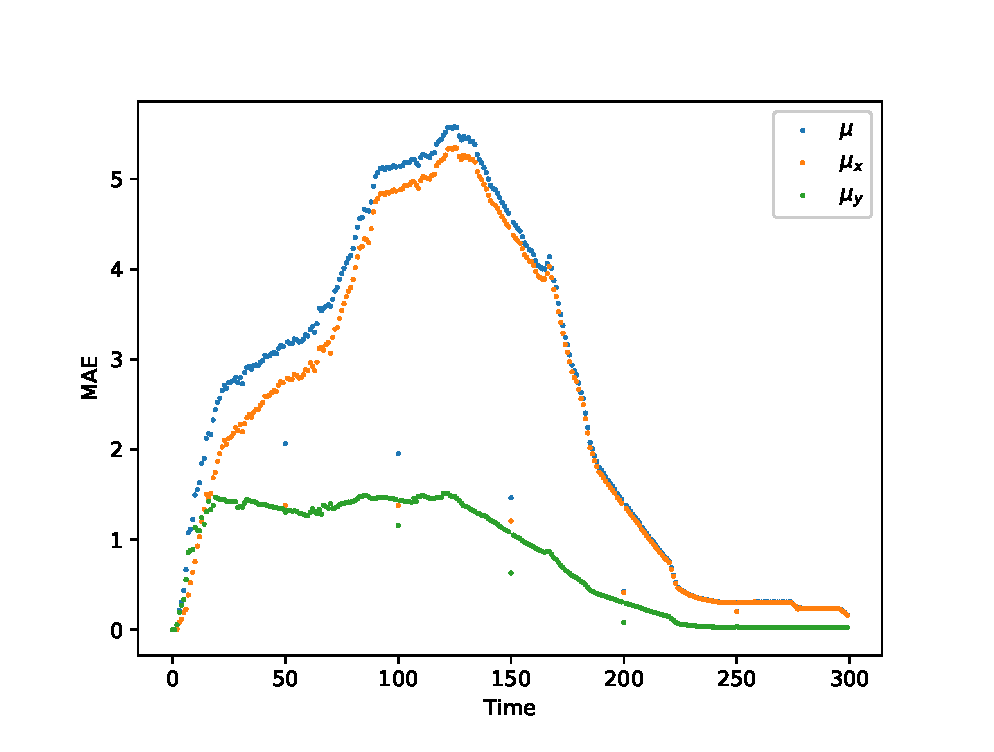
\includegraphics[width=0.8\textwidth]{errors}
    %\caption{Variation of errors with simulation time.}
    %\label{fig:errors}
%\end{figure}
